\documentclass[internal]{nhitec_design}

\usepackage{listings}

\author{ROTHEUDT Thomas et MOUCHAMPS Antoine}
\date{\today}

\title{Installation de Laravel \& Docker}

\newRem{tom}{green!60!black}

\begin{document}

\maketitle
\newpage
\tableofcontents
\newpage

\section{Introduction}
    \subsection{Qu'est-ce que Docker?}
        
        Docker est un outil open-source créé en 2012 par des français. Cet outil permet de créer, de déployer et de lancer des applications tournant dans un conteneur. Ces conteneurs sont en réalité des environnements dans lesquels les applications tournent.
        Ils sont créés grâce à des images qui sont des fichiers dockers, ainsi n'importe quel conteneur est assuré de tourner sur n'importe quel machine sans se soucier des configurations locales.\\
        L'outil est tellement populaire que les mainteneurs de librairies ou de logiciels maintiennent des images docker (dans notre cas on verra que Laravel Sail possède une image docker qui est maintenue à jour régulièrement)
        Il permet donc de "centraliser" l'environment sur lequel une application est développée. 

        \begin{figure}[h]
            \centering
            \begin{subfigure}[b]{0.3\textwidth}
                
\includegraphics[scale=0.4]{Images_formation/LogoDocker.png}
            \end{subfigure}%
        \end{figure}
        
    \subsection{Pourquoi Docker?}

        Un conteneur docker possède de nombreux avantages comparé aux machines virtuels. Premièrement, il utilise les ressources d'un système plus éfficacement qu'une VM tout en gardant ses avantages (isolation et reproductibilité). 

        \begin{wrapfigure}{l}{0.18\textheight}
            \centering
            
\includegraphics[width=0.2\textwidth]{Images_formation/Iconconteneur.png}
        \end{wrapfigure}

        Il garanti d'être identique quel que soit le système, ainsi chaque membres d'un projet est certain de travailler sur le même environment sans se soucier de la portabilité de l'application sur l'environment final.
        
        Les conteneurs sont isolés de la machine hôte, ainsi vous pouvez avoir plusieurs versions différentes de dépendances pour plusieurs projets.

        Enfin, la modifications d'un conteneurs est extrêmement simplifié comparé à une VM où les mises à jour sont souvent complexes et laborieuse.

        Pour résumer, un conteneur docker est flexible, léger, portable.

        
\newpage

    \subsection{Qu'est-ce que Laravel Sail?}
        
        Laravel Sail est une interface de ligne de commande légère pour interagir avec l'environnement de développement Docker par défaut de Laravel. 
        
        \begin{wrapfigure}{l}{0.2\textwidth}
            \centering
            
\includegraphics[width=0.2\textwidth]{Images_formation/LaravelLogo.png}
        \end{wrapfigure}
        
        Sail est un excellent point de départ pour construire une application Laravel en utilisant PHP, MySQL et Redis sans avoir besoin d'une expérience préalable de Docker.

        Au cœur de Sail se trouve le fichier docker-compose.yml et le script sail qui est stocké à la racine de votre projet. Le script sail fournit une CLI (command line interface) avec des méthodes pratiques pour interagir avec les conteneurs Docker définis par le fichier docker-compose.yml.

        Laravel Sail est pris en charge sur macOS, Linux et Windows (via WSL2).

        Pour résumer, le scrip sail permet de gérer le projet Laravel à l'intérieur du conteneur du projet. De plus Laravel Sail est complètement compatible avec Docker, ce qui permet des interactions plus simples avec les conteneurs.

\section{Installation de Docker}
    \subsection{Installation Linux}

        \begin{figure}[h]
            \centering
            
\includegraphics[scale=0.05]{Images_formation/LinuxLogo.png}
        \end{figure}

        L'Installation linux nécéssite de suivre quelques étapes de plus que pour l'Installation MacOS ou Windows.\\
        \begin{itemize}
     
            \item[1.] Mettez à jour l'index des paquets apt et des paquets d'installation pour permettre à apt d'utiliser un dépôt sur HTTPS:
            
                \begin{lstlisting}
                    sudo apt-get update
                \end{lstlisting}

            \item[2.] Installez les dépendances de Docker:

                \begin{lstlisting}
                    sudo apt-get install \
                        ca-certificates \
                        curl \
                        gnupg \
                        lsb-release
                \end{lstlisting}

\newpage

            \item[3.] Ajoutez la clé GPG officielle de Docker:

                \begin{lstlisting}
                    sudo mkdir -m 0755 -p /etc/apt/keyrings

                    curl -fsSL https://download.docker.com/linux/ubuntu/gpg | 
                    sudo gpg --dearmor -o /etc/apt/keyrings/docker.gpg
                \end{lstlisting}

            \item[4.] Configurez le répertoire:\\

                \begin{footnotesize}
                    \textit{\textdollar(lsb\_release -cs)} doit dans quelques cas être remplacé par votre version de distribution linux.\\
                    Dans l'installation de référence on a remplacé par \textit{jammy}.
                \end{footnotesize}
                \begin{lstlisting}
                    echo \
                    "deb [arch=\$(dpkg --print-architecture) 
                    signed-by=/etc/apt/keyrings/docker.gpg] https://download.docker.com/linux/ubuntu \
                    \$(lsb_release -cs) stable" 
                    | sudo tee /etc/apt/sources.list.d/docker.list > /dev/null
                \end{lstlisting}

            \item[5.] Verifiez que le répertoire est bien configurer:

                \begin{lstlisting}
                    sudo apt-get update
                \end{lstlisting}    

            \item[6.] Installez Docker Engine, conteneurd, et Docker Compose:

                \begin{lstlisting}
                    sudo apt-get install docker-ce docker-ce-cli 
                    conteneurd.io docker-buildx-plugin docker-compose-plugin
                \end{lstlisting}
                \begin{footnotesize}
                    Vous pouvez tester votre installation avec la commande: \textit{sudo docker run hello-world}
                \end{footnotesize}

                \bigskip
            \item[7.] Installez Docker Desktop:

            
                \begin{footnotesize}
                    Téléchargez le \href{https://desktop.docker.com/linux/main/amd64/docker-desktop-4.17.0-amd64.deb?utm_source=docker&utm_medium=webreferral&utm_campaign=docs-driven-download-linux-amd64}{Docker Destop} et l'installez avec la commande:
                \end{footnotesize}

                \begin{lstlisting}
                    sudo apt-get install ./docker-desktop-<version>-<arch>.deb
                \end{lstlisting}

        \end{itemize}

\bigskip

        \begin{footnotesize}
            L'Installation de référence pour ce guide a été faite sur une distribution Linux Mint (distibution basé sur ubuntu)\\
        \end{footnotesize}

\newpage

    \subsection{Installation Windows}

        \begin{figure}[h]
            \centering
            
\includegraphics[scale=0.025]{Images_formation/WindowsLogo.png}
        \end{figure}

        Il est fortement conseillé d'utiliser \href{https://learn.microsoft.com/fr-fr/windows/wsl/install}{WSL2}. C'est une application windows permettant d'installer un environnement linux avec la distribution de votre choix nativement sous windows.
        
        \begin{itemize}
            \item[1.] Téléchargez \href{https://desktop.docker.com/win/main/amd64/Docker%20Desktop%20Installer.exe}{Docker Desktop}
            
            \item[2.] Exécutez le fichier d'installation .exe
            
            \item[3.] Vérifiez l'installation: 
            
                Lancer votre environment wsl et lancer la commande suivante:
                \begin{lstlisting}
                    docker
                \end{lstlisting}
        \end{itemize}

        Docker et wsl2 sont totalement compatibles. De plus l'utilisation de \href{https://code.visualstudio.com/docs/remote/wsl}{VSCode} est conseillé car il permet l'utilisation de l'extension docker.



    \subsection{Installation MacOS}

        \begin{figure}[h]
            \centering
            
\includegraphics[scale=0.025]{Images_formation/MacosLogo.png}
        \end{figure}

        \begin{itemize}
            \item[1.] Téléchargez Docker Desktop \href{https://desktop.docker.com/mac/main/arm64/Docker.dmg?utm_source=docker&utm_medium=webreferral&utm_campaign=dd-smartbutton&utm_location=module}{Apple Chip} ou \href{https://desktop.docker.com/mac/main/amd64/Docker.dmg?utm_source=docker&utm_medium=webreferral&utm_campaign=dd-smartbutton&utm_location=module}{Intel Chip}
            \item[2.] Installez Docker Desktop dans le dossier application
        \end{itemize}

\newpage

    \subsection{Aperçu}

        Si tout s'est bien passé vous êtes en mesure de lancer Docker Desktop. 
        Vous avez donc le panneau de contrôle de Docker Desktop qui devrait ressembler à ça:\\
        
        \begin{figure}[h]
            \centering
            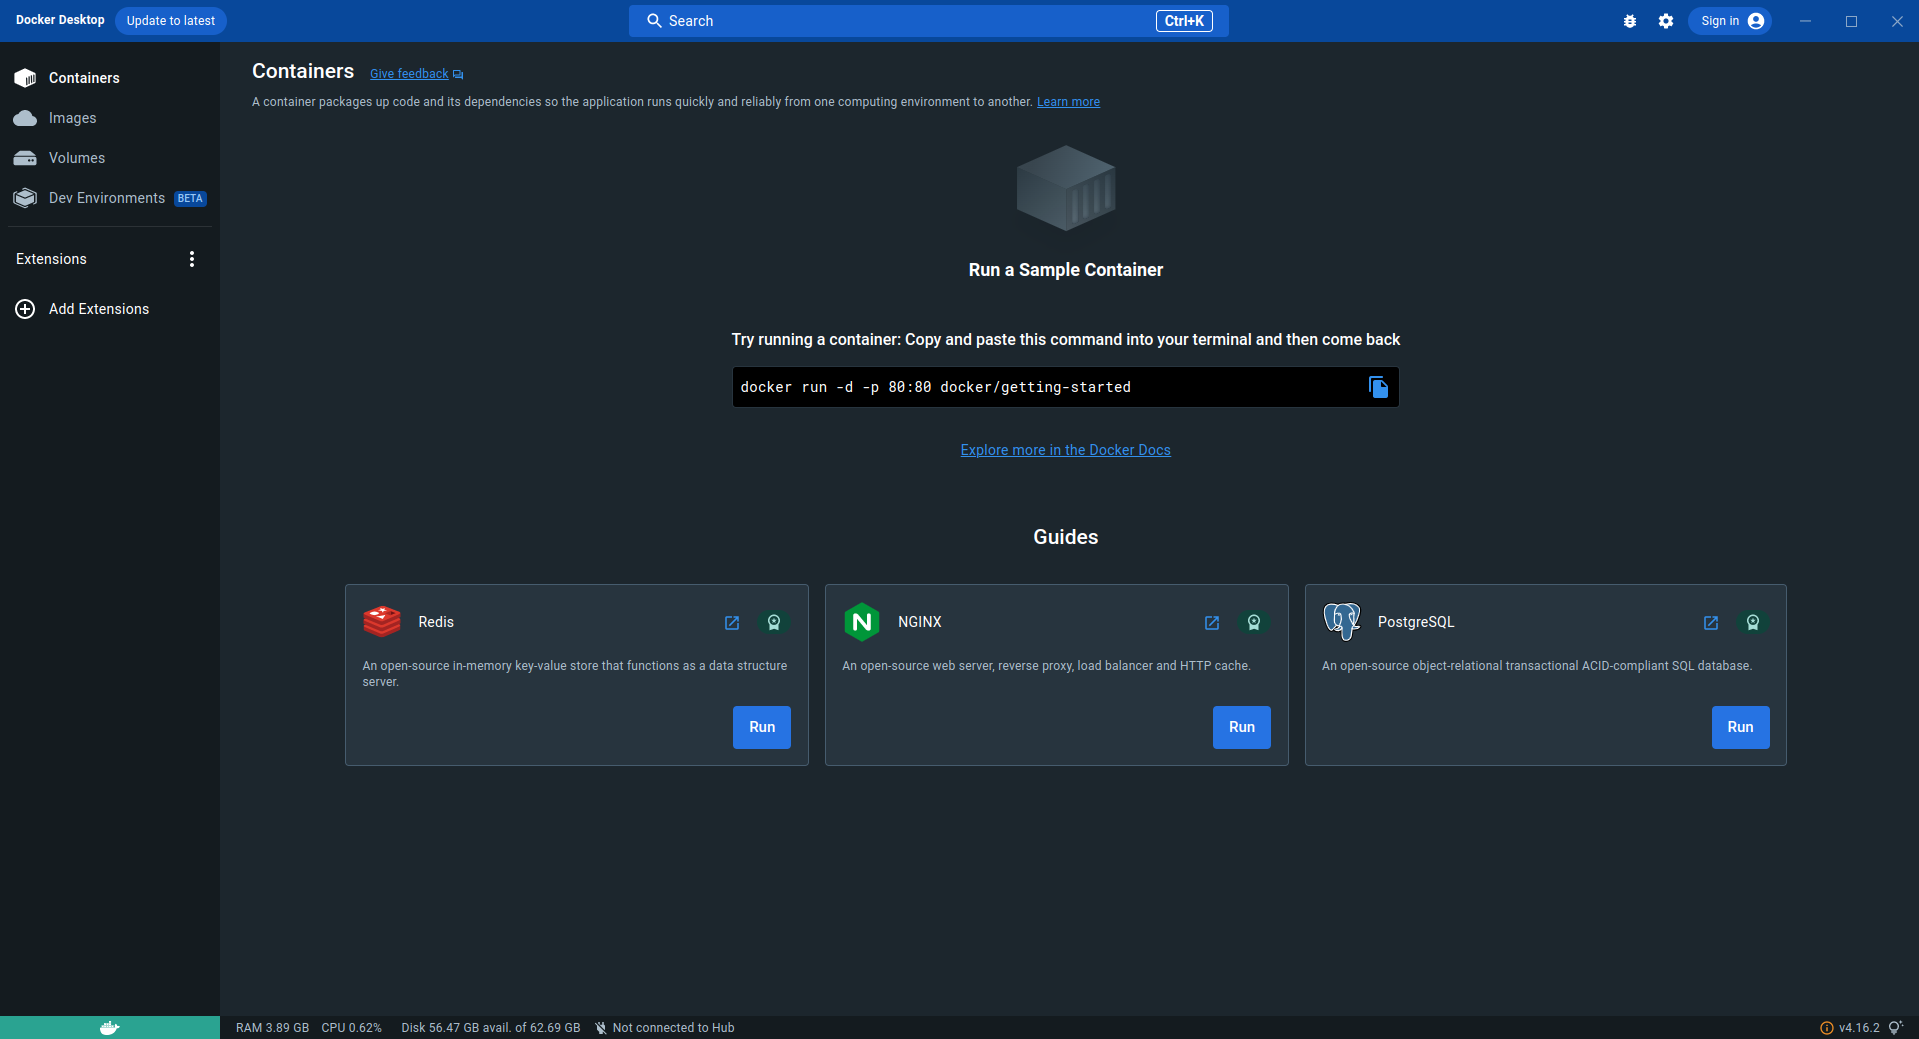
\includegraphics[scale=0.25]{Images_formation/PanelDocker.png}
        \end{figure}

        Vous pouvez voir différents onglets sur la gauche:

        \begin{itemize}
            \item[] Conteneurs: Cet onglet va contenir tous les conteneurs que vous avez créés\\
            \item[] Images: Cet onglet va contenir toutes les images d'installation des services installés dans nos conteneurs\\
            \item[] Volumes: Cet onglet contient les volumes liés aux services qui contiennent les data de nos applications\\
            \item[] Dev Environnements: une feature très intéressante permettant de créer des environnements de développement \footnotesize{\href{https://docs.docker.com/desktop/dev-environments/}{plus d'informations}}
        \end{itemize}

\newpage

\section{Création Projet Laravel}

    \subsection{Création du dossier}
        Pour créer un nouveau projet laravel dans un dossier "exemple-app" il suffit juste d'entrer la ligne de commande:

        \begin{lstlisting}
            curl -s https://laravel.build/example-app | bash
        \end{lstlisting}

        Avec cette commande votre projet sera installé avec plusieurs services de base (mysql, redis, et d'autres)

        il est possible de choisir les services à installer avec le mot clé \textit{with}

        \begin{lstlisting}
            curl -s "https://laravel.build/example-app?with=mysql,redis" | bash
        \end{lstlisting}
        Mais pour plus de claireté, on va utiliser la première commande.

        une fois lancé le projet va se créer (cela peut prendre un certain temps)

        \begin{figure}[h]
            \centering
            \begin{subfigure}{0.3\textwidth}
                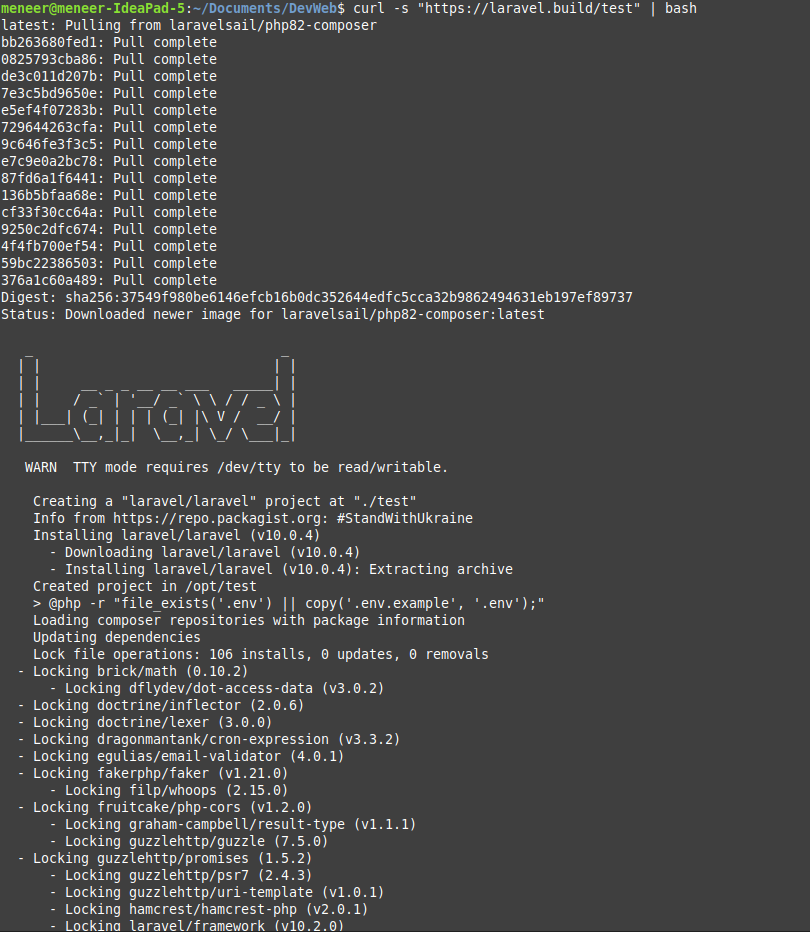
\includegraphics[width=\textwidth]{Images_formation/CreateProject.png}
            \end{subfigure}
            \begin{subfigure}{0.3\textwidth}
                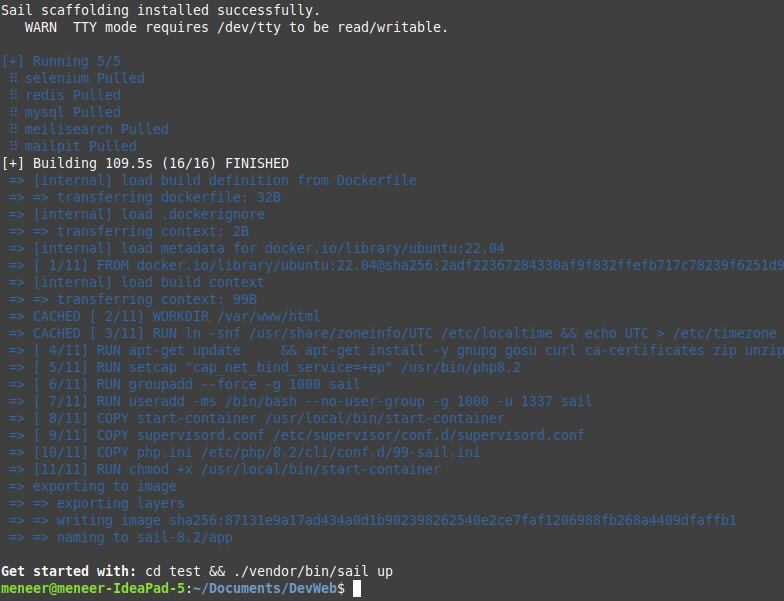
\includegraphics[width=\textwidth]{Images_formation/CreateProject2.png}
            \end{subfigure}
        \end{figure}


        Une fois le dossier du projet créé vous allez rentrer dans le Dossier et ouvrir le fichier \textit{docker-compose.yml}.

        Ce fichier représente la configuration générale de votre conteneur, c'est ici que l'on va définir les services à installer, les versions, les images, ect.
        Ce fichier est très important, sans lui, pas de conteneur.

        Vous pouvez voir qu'il est composé de plusieurs \href{https://docs.docker.com/compose/compose-file/}{section}, \textit{Version, services, network, volumes}. Chaque section à son utilitée. Nous allons nous concentrer sur la section service du fichier. Plus précisement, nous allons ajouter un service.\\ 


\newpage

    \subsection{Ajout PhpMyAdmin}

        On va ajouter un service à notre projet qui est nécessaire à la gestion de notre base de donnée,\\ \textit{PhpMyAdmin}.
        
        Pour ce faire, rendez-vous à la fin de la section \textit{services}, et ajoutez y \textit{PhpMyAdmin} comme suit:

        \begin{lstlisting}
            phpmyadmin:
                image: 'phpmyadmin:latest' 
                ports:
                    - '8080:80' 
                networks:
                    - sail 
                environment:
                    - PMA_ARBITRARY=1
        \end{lstlisting}

        Une fois cela fait, PhpMyAdmin est intégré au projet.

    \section{Utilisation}
    Pour utiliser le script, il vous faudra utiliser la commande suivante dans le dossier du projet (sail est installé par defaut lors de la création du projet):

    \begin{lstlisting}
        ./vendor/bin/sail [command] [options] [arguments]
    \end{lstlisting}

    Vous pouvez créer un alias pour sail en ajoutant la ligne suivante à votre .bashrc, zshrc, ect: 

    \begin{lstlisting}
        alias sail='[ -f sail ] && sh sail || sh vendor/bin/sail'
    \end{lstlisting}
    
    \subsection{Démarrage du container}
        Pour lancer le container et ainsi pouvoir travailler sur le projet, entrez dans le dossier de votre projet via un terminal et lancer la commande:
        
        \begin{lstlisting}
            sail up -d
        \end{lstlisting}

        Cette commande lancera le container en mode détacher pour garder l'accès au terminal (pratique si l'on travaille sur VSCode)\\
        \footnotesize{On peut aussi lancer dans un terminal avec \textit{sail up}}


        Vous pouvez maintenant avoir accès à la page de votre projet en allant sur \textit{localhost} via un moteur de recherche comme Mozilla, Google, ect.

    \subsection{Arrêt du container}

    Pour éteintre le container lorsque vous avez finis de travailler, tapez la commande

    \begin{lstlisting}
        sail down
    \end{lstlisting}
    \end{document}
